\documentclass{guide}

\title{GPIO en Breadboards}
\author{Jorn Bunk}
\level{1}

\begin{document}
\section{GPIO pinnen}
Voor het miniproject van CSN gaan jullie aan de slag met de Raspberry Pi. Jullie zullen deze gebruiken om knopjes, LEDs, en mogelijk andere electronica aan te sturen. Het verbinden van deze onderdelen met de Pi gebeurt via de GPIO pinnen: de 40 pinnen linksboven op de Pi. Al deze pinnen hebben een vaste functie: een aantal pinnen levert een vast voltage ($3,3V$ of $5V$) en dient als \enquote{plus}, een aantal pinnen is met de \enquote{ground} ($0V$) verbonden en dient als \enquote{min}, en de rest is als GPIO pin vanuit Python aan te spreken. In Figuur~\ref{fig:pinout} is te zien welke pin waarvoor gebruikt kan worden. Een deel van de GPIO pinnen heeft een speciale functie (bijvoorbeeld \enquote{UART0\_TXD}), maar dit mag je voor nu negeren.

Let er op dat pinnen op twee manieren zijn gelabeled: ze hebben zowel een nummer dat aangeeft waar de pin zich bevindt (het physical pinnummer) als een nummer dat als naam gebruikt wordt (het BCM pinnummer). De fysieke pin 8 komt bijvoorbeeld overeen met het label \enquote{GPIO14} of \enquote{BCM14}. Als het niet lukt een pin vanuit Python aan te spreken dan heb je mogelijk het verkeerde nummeringsschema gebruikt.

\begin{figure}[h]
  \centering
  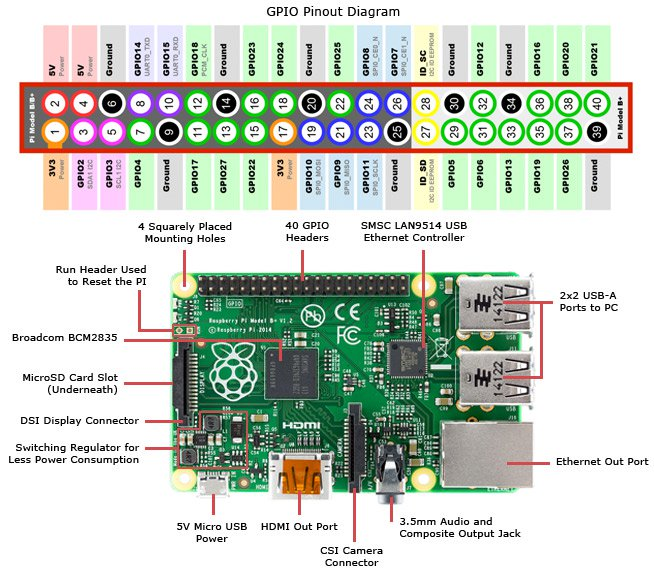
\includegraphics[width=\textwidth]{images/pinout.png}
  \caption{Pinout van de Raspberry Pi (bron: \href{https://www.jameco.com/Jameco/workshop/circuitnotes/raspberry-pi-circuit-note.html}{Jameco}).} \label{fig:pinout}
\end{figure}

\section{Breadboard}
De LEDs en knoppen zijn met behulp van draadjes (jumper wires) aan te sluiten, deze zijn te vinden in de tweede lade van de TI Labshop. De verschillende onderdelen zijn echter bedoeld om op een printplaat te solderen, niet om met draadjes aan elkaar geknoopt te worden. Een alternatief voor soldern is de breadboard: een plastic bordje met gaten die per rij aan elkaar verbonden zitten. Je kunt hier alle onderdelen inprikken om deze met elkaar te verbinden. In de TI Labshop zijn verschillende maten te koop, voor prijzen van \euro 0,70 tot \euro 2,10. Afhankelijk van de maat heb je een aantal rijen waarbij ieder gat in een rij met elkaar in verbinding staat. In het midden zit een richel, waardoor de rijen onderbroken zijn. Grotere breadboards hebben daarnaast aan de buitenkant twee lange rijen waarvan rood voor de VCC ($3,3V$ of $5V$) en blauw voor de GND ($0V$) bedoeld zijn.


\begin{figure}[h]
  \centering
  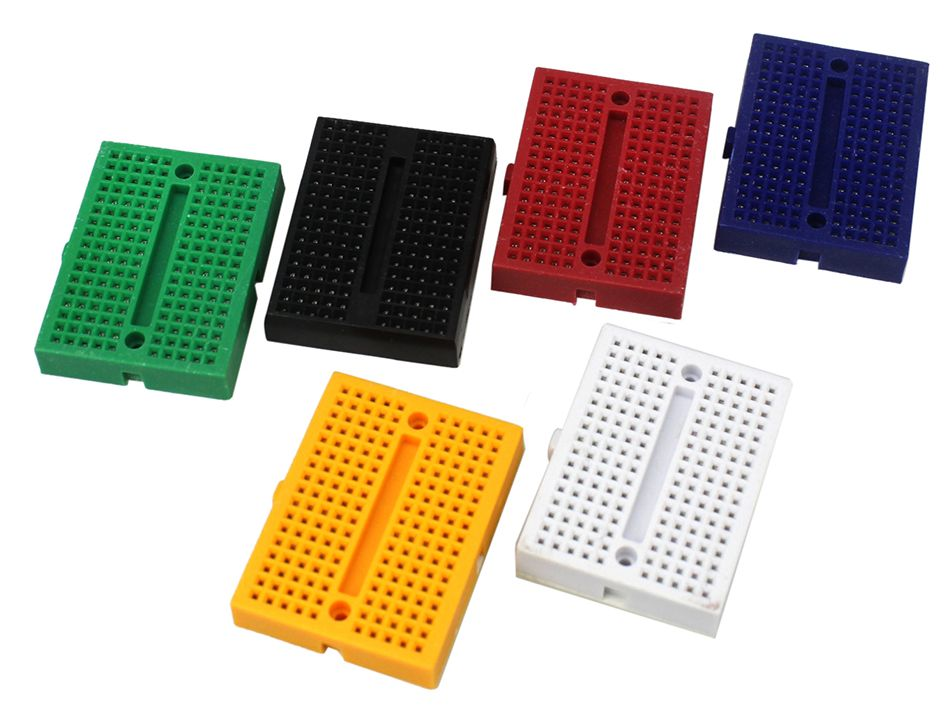
\includegraphics[width=8cm]{images/bbsmall.png}
  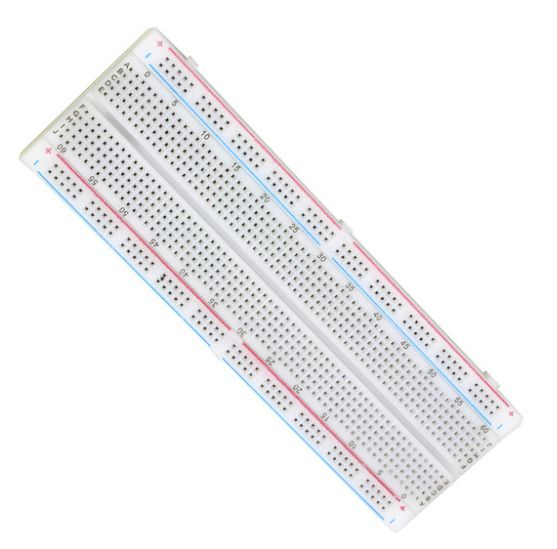
\includegraphics[width=8cm]{images/bblarge.png}
  \caption{Verschillende breadboards (bron: \href{http://technische-informatica.nl/ti-lab-shop}{TI Labshop}).} \label{fig:breadboards}
\end{figure}

\end{document}
